%!TEX root = ../dokumentation.tex
%%%%%%%%%%%%%%%%%%%%%%%%%%%%%%%%%%%%%%%%%%%%%%%%%%%%%%%%%%%%%%%%%%%%%%%%%%%%%%%%%%%%%%%%%
\chapter{Entwicklung des Modells}\label{sec:model}

Als ersten Schritt zur Erkennung von Objekten im Straßenverkehr wird der Entwurf eines \ac{CNN} angeführt. Maßgeblichen Einfluss auf die Entscheidung der Architektur des \ac{CNN} sowie der Vorgehensweise hat die Arbeit \citetitle{rock_paper_scissors} \cite{rock_paper_scissors}. Das Modell wird als beispielhafte Implementierung einer \gls{mc_classification} entworfen und bietet somit die Möglichkeit einer theoretischen Transformation in eine \gls{ml_classification}. Als Datensatz wird der \ac{CIFAR}-10 Datensatz verwendet. Der \acs{CIFAR}-10-Datensatz ist eine Sammlung von Bildern, die üblicherweise zum Trainieren von Algorithmen für maschinelles Lernen und Computer Vision verwendet werden. Bestehend aus 60000 32x32 Farbbildern, unterteilt in 10 Klassen, ist es einer der am häufigsten verwendeten Datensätze für die Forschung zum maschinellen Lernen \cites{most_used_datasets_2}{most_used_datasets}. Das Test-Batch enthält 1000 zufällig ausgewählte Bilder jeder Klasse, wohingegen der Train-Batch die restlichen 5000 Bilder einer jeden Klasse enthält \cites{cifar10}{cifar10_2}.

\section{Vorverarbeitung der Daten}

\citeauthor{Goodfellow2016} erwähnen in ihrem Buch \citetitle{Goodfellow2016} die Problematik des Overfittings von Neuronalen Netzen. 

\begin{quote}
	 The central challenge in machine learning is that we must perform well on new, previously unseen inputs — not just those on which our model was trained. The ability to perform well on previously unobserved inputs is called generalization \cite[110]{Goodfellow2016}. 
\end{quote}

Um dem Overfitting Effekt des \ac{CNN} vorzubeugen, wird der gewählte Datensatz zunächst einer Reihe von Augmentationsalgorithmen unterzogen. Diese Schritte sind notwendig für die Sicherstellung eines generalisierten Ansatzes zur Erkennung neuer Test-Splits. Dabei lernt das Modell von bekannten Beispielen und kann somit verallgemeinert auf neue Beispiele in der Zukunft eingesetzt werden. 
\newpage
\subsection{Ausrichtung des Bildtensors}

Der erste Schritt der Augmentation ist die zufällige Veränderung der Ausrichtung des Bildes. TensorFlow bietet passend hierfür zwei Funktionen an, die eine Spiegelung an horizontaler bzw. vertikaler Achse vornehmen.

\vspace*{10mm}

\begin{lstlisting}[caption={Python Funktion zum zufälligen Ändern der Ausrichtung}]
	def flip_c(image: tf.Tensor) -> tf.Tensor:
    # Randomize alignment (left/right)
    image = tf.image.random_flip_left_right(image)
    # Randomize alignment (top/down)
    image = tf.image.random_flip_up_down(image)
    # Return the randomized image
    return image
\end{lstlisting}

Die Funktion \emph{random\_flip\_left\_right} gibt mit einer Wahrscheinlichkeit von 1 zu 2 den Inhalt des Bildes gespiegelt entlang der zweiten Dimension, also der Breite, aus. Andernfalls wird das Bild so ausgegeben, wie es ist. Wenn ein Stapel von Bildern übergeben wird, wird jedes Bild unabhängig von den anderen Bildern zufällig gespiegelt \cite{tf_r_f_l_r}. Die Funktion \emph{random\_flip\_up\_down} gibt mit derselben Wahrscheinlichkeit ein gespiegeltes Bild entlang der ersten Dimension zurück \cite{tf_r_f_u_d}. 

\begin{figure}[htb]
	\begin{subfigure}[ht]{.5\textwidth}
		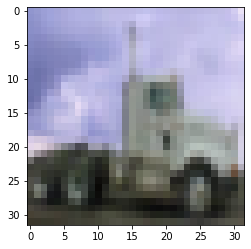
\includegraphics[width=\textwidth]{images/flip}
		\caption{Initiales Bild}
		\label{fig:flip}
	\end{subfigure}\hfill%
	\begin{subfigure}[ht]{.5\textwidth}
		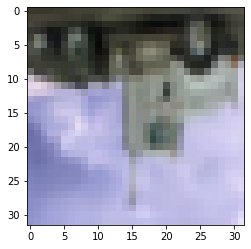
\includegraphics[width=\textwidth]{images/flip_a}
		\caption{Bild nach Flip-Augmentation}
		\label{fig:flip_a}
	\end{subfigure}\hfill%
	\caption{Vergleich desselben Bildes nach Randomisierung der Ausrichtung}
\end{figure}

\subsection{Farbanpassung des Bildtensors}

Als weiterer Bestandteil des Augmentationsprozesses werden zufällige Werte für Farbton, Sättigung, Helligkeit und Kontrast gewählt. 
Der Farbton wird anhand eines übergebenen Deltas im Interval $[0,0.08]$ modifiziert \cite{tf_r_hue}. Die Sättigung des Bildes wird im Interval $[0.7,1.3]$ angepasst \cite{tf_r_saturation}. Ein ebenso wichtiger Bestandteil der Farbaugmentation ist die Anpassung der Helligkeit, welche in diesem Fall mit Hilfe des Intervals $[0,0.05]$ angepasst wird \cite{tf_r_brightness}. Abschließend wird eine Modifikation des Kontrastes im Interval $[0.8,1]$ durchgeführt \cite{tf_r_contrast}. 

\vspace*{10mm}

\begin{lstlisting}[caption={Python Funktion zum zufälligen Ändern des Farbwertes}]
	def color_c(image: tf.Tensor) -> tf.Tensor:
    # Randomize hue
    image = tf.image.random_hue(image, max_delta=0.08)
    # Randomize saturation
    image = tf.image.random_saturation(image, lower=0.7, upper=1.3)
    # Randomize brightness
    image = tf.image.random_brightness(image, 0.05)
    # Randomize contrast
    image = tf.image.random_contrast(image, lower=0.8, upper=1)
    # Return the randomized image
    return image
\end{lstlisting}

\begin{figure}[htb]
	\begin{subfigure}[ht]{.5\textwidth}
		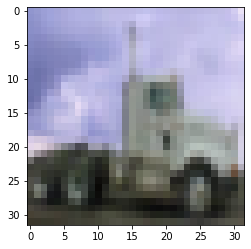
\includegraphics[width=\textwidth]{images/flip}
		\caption{Initiales Bild}
		\label{fig:color}
	\end{subfigure}\hfill%
	\begin{subfigure}[ht]{.5\textwidth}
		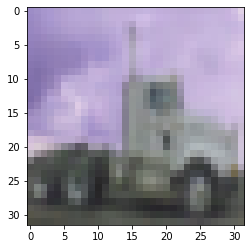
\includegraphics[width=\textwidth]{images/color_a}
		\caption{Bild nach Farbaugmentation}
		\label{fig:color_a}
	\end{subfigure}\hfill%
	\caption{Vergleich desselben Bildes nach Randomisierung der Farbwerte}
\end{figure}

\subsection{Rotation des Bildtensors}

Zur weiteren Unterbindung des Overfittings wird ein Verfahren zur Rotation des Bildtensors eingesetzt. TensorFlow bietet hierzu in der zugehörigen Bildbibliothek eine Funktion zur 90-Grad Rotation an \cite{tf_r_rot90}. Über einen Parameter lässt sich die Anzahl der Rotationsschritte bestimmen, woraus eine zufällige Rotation entsteht. Die dynamische Erzeugung von Rotationsschritten wird mittels der Funktion \emph{tf.random.uniform} generiert, welche einen Zufallswert aus einer Gleichverteilung ausgibt \cite{tf_r_uniform}.

\vspace*{10mm}

\begin{lstlisting}[caption={Python Funktion zum zufälligen Rotieren des Bildtensors}]
	def rotation_c(image: tf.Tensor) -> tf.Tensor:
    # Rotate 0, 90, 180, 270 degrees
    # Return the randomized image
    return tf.image.rot90(
        image,
        tf.random.uniform(shape=[], minval=0, maxval=4, dtype=tf.int32)
    )
\end{lstlisting}

\begin{figure}[htb]
	\begin{subfigure}[ht]{.5\textwidth}
		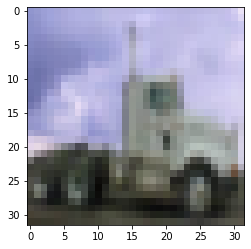
\includegraphics[width=\textwidth]{images/flip}
		\caption{Initiales Bild}
		\label{fig:rotate}
	\end{subfigure}\hfill%
	\begin{subfigure}[ht]{.5\textwidth}
		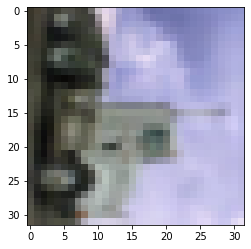
\includegraphics[width=\textwidth]{images/rotate_a}
		\caption{Bild nach Augmentation der Rotation}
		\label{fig:rotate_a}
	\end{subfigure}\hfill%
	\caption{Vergleich desselben Bildes nach Randomisierung der Rotation}
\end{figure}

\subsection{Inversion des Bildtensors}

Um einen noch größeren Grad der variablen Gestaltung einzelner Bildtensoren zu erreichen, wird von dem übergebenen Tensor, mit einer Wahrscheinlichkeit von 1 zu 2, die Inverse gebildet und zurückgegeben. 

\vspace*{10mm}

\begin{lstlisting}[caption={Python Funktion zum zufälligen Rotieren des Bildtensors}]
	def inversion_c(image: tf.Tensor) -> tf.Tensor:
  	# Invert the submitted tensor
    random = tf.random.uniform(shape=[], minval=0, maxval=1)
    if random > 0.5:
        image = tf.math.multiply(image, -1)
        image = tf.math.add(image, 1)
    # Return the randomized image
    return image
\end{lstlisting}



\begin{figure}[htb]
	\begin{subfigure}[ht]{.5\textwidth}
		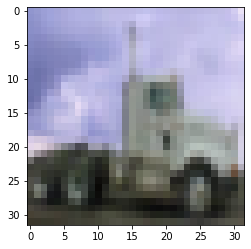
\includegraphics[width=\textwidth]{images/flip}
		\caption{Initiales Bild}
		\label{fig:inversion}
	\end{subfigure}\hfill%
	\begin{subfigure}[ht]{.5\textwidth}
		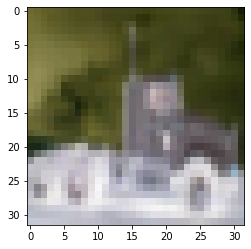
\includegraphics[width=\textwidth]{images/inversion_a}
		\caption{Bild nach Inversion des Farbraums}
		\label{fig:inversion_a}
	\end{subfigure}\hfill%
	\caption{Vergleich desselben Bildes nach Inversion des Farbraums}
\end{figure}
\newpage
\subsection{Finale Augmentation des Bildtensors}

Nach der Definition aller Augmentationsfunktionen können diese auf den eigentlichen Bildtensor angewandt werden. 
\vspace*{10mm}
\begin{lstlisting}[caption={Finaler Augmentationsschritt}]
	def augment_c(image, label):
  	# Randomize alignment
  	image = flip_c(image)
  	# Randomize color (saturation/hue/brightness/contrast)
  	image = color_c(image)
  	# Randomize rotation
  	image = rotation_c(image)
  	# Randomize inversion
  	image = inversion_c(image)
  	# Return the fully randomized image
  	return image, label
\end{lstlisting}

Dieser Schritt fasst die zuvor definierten Schritte zusammen und gibt die modifizierte Version des Bildtensors zurück, wie in Abbildung \ref{fig:augmented} zu sehen ist. Die Schwierigkeit des Erkennens durch das menschliche Auge ist gewollt, da hierdurch die Fähigkeit einer Generalisierung des Netzwerks geschmälert wird. 

\begin{figure}[htb]
	\centering
	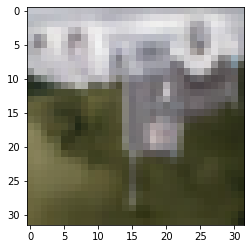
\includegraphics{images/augmented.png}
	\caption{Darstellung des Bildtensors nach vollständiger Augmentation}
	\label{fig:augmented}
\end{figure}

\section{Entwurf eines Netzwerks zur Klassifikation von Objekten}

Künstliche neuronale Netze haben zwei Haupt-Hyperparameter, die die Architektur oder Topologie des Netzes steuern: die Anzahl der Schichten und die Anzahl der Knoten in jeder versteckten Schicht. Diese Werte müssen während des Architekturentwurfs definiert werden und sind zur Trainingszeit des Netzwerks nicht veränderbar. Der zuverlässigste Weg der Hyperparametersuche ist ein systematisches Experimentieren mit iterativer Validierung \cite{hyperparameter_cnn}. Es ist gängige Praxis mit einem Grundmodell anzufangen und dieses Schritt-für-Schritt anzupassen. Als Grundmodell wird das Sequentielle Modell eingesetzt, kombiniert mit einem Convolutional2D-Layer, welcher die räumliche Faltung des Bildtensors realisiert (siehe Kapitel \ref{sec:cnn}). Mit Hilfe des Flatten-Layers wird die Dimensionalität aus dem Netzwerk genommen, woraus ein Layer mit $32x32x32 = 32768$ Neuronen entsteht. Die Ausgabe des Netzwerks wird durch einen Dense-Layer realisiert, der die 10 Ausgabeneuronen anhand der Softmax Aktivierungsfunktion bewertet (siehe Kapitel \ref{sec:ann}). Abbildung \ref{fig:basemodell} zeigt das Modell in der Architekturansicht. 

\begin{figure}[htb]
	\centering
	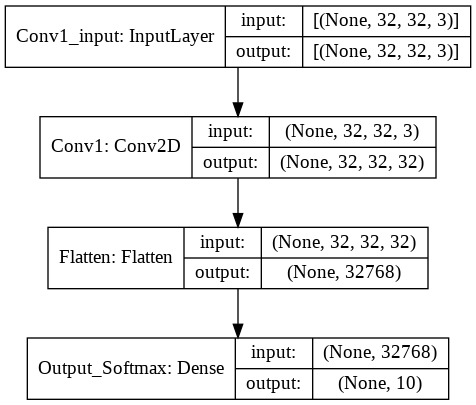
\includegraphics[width=0.5\textwidth]{images/model1}
	\caption{Architektur des Grundmodells}
	\label{fig:basemodell}
\end{figure}

\begin{figure}[htb]
	\centering
	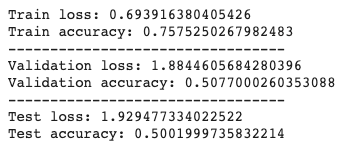
\includegraphics[width=0.5\textwidth]{images/model1_scores}
	\caption{Verlust- und Genauigkeitskennzahlen des Grundmodells}
	\label{fig:model1_scores}
\end{figure}

Das zuvor gezeigte Modell erzielt auf den Trainings-, Test- und Validierungsdatensätzen die in Abbildung \ref{fig:model1_scores} aufgezeigten Verlust- und Genauigkeitskennzahlen. Die erhobenen Metriken zeigen die Dringlichkeit einer Anpassung des Modells auf. Die erzielte Genauigkeit des Trainings ist mit einem Score von 0.75 zunächst in Ordnung, jedoch zeigen die Validierungs- und Test Genauigkeit eine starke Abweichung zu diesem Wert auf. Damit eine Verbesserung der einzelnen Werte erzielt werden kann, wird im nächsten Schritt die Architektur analysiert. Hierfür wird die Anzahl der Schichten evaluiert und Anpassungen von Hyperparametern vorgenommen. 

\subsection{Evaluierung der Anzahl an Convolutional Layers}
Um die Anzahl an Convolutional Layers mit der besten Genauigkeit ermitteln zu können, erfolgt eine Evaluierung vier unterschiedlicher Modellarchitekturen. \citeauthor{ChrisDeotte2018} führt die Grundidee in der Publikation \citetitle{ChrisDeotte2018} ein \cite{ChrisDeotte2018}.
Die vier Modelle werden wie folgt klassifiziert:
\begin{itemize}
	\item 2432 - \textbf{$[$32C5-P2$]$} - 256 - 10
	\item 2432 - \textbf{$[$32C5-P2$]$} - \textbf{$[$48C5-P2$]$} - 256 - 10
	\item 2432 - \textbf{$[$32C5-P2$]$} - \textbf{$[$48C5-P2$]$} - \textbf{$[$64C5-P2$]$} - 256 - 10
	\item 2432 - \textbf{$[$32C5-P2$]$} - \textbf{$[$48C5-P2$]$} - \textbf{$[$64C5-P2$]$} - \textbf{$[$80C5-P2$]$} - 256 - 10
\end{itemize}

Die Notation lässt sich folgendermaßen erklären: 2432 - Anzahl der Eingabeneuronen; $[\Delta$C5-P2$]$ - Convolutional Layer mit $\Delta$ Filtern und anschließendem MaxPooling Layer der Größe 2, Kernel-Größe von 5 und einem Stride von 2; 256 - Fully-connected Dense Layer mit 256 Einheiten; 10 - Ausgabeneuronen zur Klassifikation der Labels. 

Die Verwendung von genau vier Modellen in dieser Evaluierung lässt sich auf die Eingabegröße des Bildes zurückführen. Das Eingabebild besitzt die Größe $32x32$. Nach der Ersten Faltung ist die Größe auf $16x16$ reduziert. Die Zweite Faltung verringert dies auf $8x8$, nach der Dritten besitzt das Bild lediglich eine Größe von $4x4$. Kompiliert werden die Modelle mit Hilfe des \gls{Adam}-Optimizers \cite{kingma2017adam} und der Sparse-Categorical-Crossentropy Verlustfunktion \cite{scc-2021}.

\begin{figure}[htb]
	\centering
	\begin{subfigure}[ht]{.9\textwidth}
		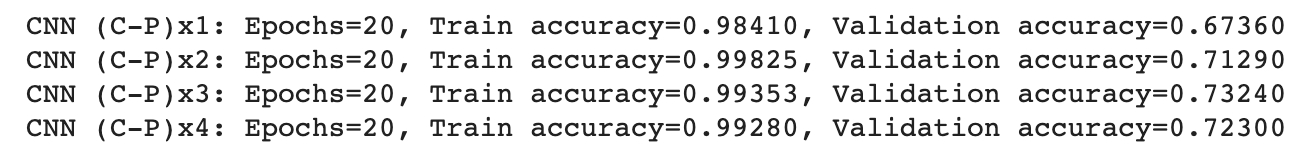
\includegraphics[width=\textwidth]{images/convlayers_result}
		\caption{Genauigkeitsmetriken unterschiedlicher \ac{CNN} Architekturen}
		\label{fig:convlayer_results}
	\end{subfigure}\hfill%
	\begin{subfigure}[ht]{.9\textwidth}
		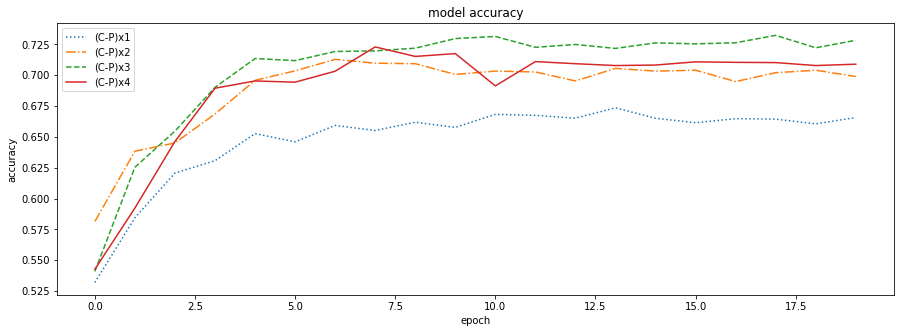
\includegraphics[width=\textwidth]{images/convlayers_result_graph}
		\caption{Grafische Darstellung der Genauigkeitsmetriken}
		\label{fig:convlayer_graph_results}
	\end{subfigure}\hfill%
	\caption{Entscheidungsfindung \ac{CNN} Architektur}
\end{figure}

Aus den in Abbildung \ref{fig:convlayer_results} und \ref{fig:convlayer_graph_results} zu entnehmenden Metriken lässt sich die beste Genauigkeit bei dem Modell \textbf{(C-Px3)} erkennen, was auf die Verwendung von drei Convolutional Layers schließen lässt. Die gewonnene Erkenntnis kann somit im nächsten Schritt übernommen und als neues Grundmodell verwendet werden. 

\subsection{Evaluierung der Feature-Map Größe}

Die Feature-Map gibt an, wie hoch die Dimensionalität des Ausgangsraumes ist (d.h. die Anzahl der Ausgangsfilter in der Faltung) \cite{conv2d-2021B}. Für eine aussagekräftige Statistik der Feature-Map Größe wird das zuvor neu definierte Grundmodell weitergehend modifiziert. Dabei werden folgende Netzwerke evaluiert:

\begin{itemize}
	\item 2432 - $[$\textbf{8}C5-P2$]$ - $[$\textbf{16}C5-P2$]$ - $[$\textbf{24}C5-P2$]$ - 256 - 10
	\item 2432 - $[$\textbf{16}C5-P2$]$ - $[$\textbf{32}C5-P2$]$ - $[$\textbf{48}C5-P2$]$ - 256 - 10
	\item 2432 - $[$\textbf{24}C5-P2$]$ - $[$\textbf{48}C5-P2$]$ - $[$\textbf{72}C5-P2$]$ - 256 - 10
	\item 2432 - $[$\textbf{32}C5-P2$]$ - $[$\textbf{64}C5-P2$]$ - $[$\textbf{96}C5-P2$]$ - 256 - 10
	\item 2432 - $[$\textbf{40}C5-P2$]$ - $[$\textbf{80}C5-P2$]$ - $[$\textbf{120}C5-P2$]$ - 256 - 10
	\item 2432 - $[$\textbf{48}C5-P2$]$ - $[$\textbf{96}C5-P2$]$ - $[$\textbf{144}C5-P2$]$ - 256 - 10
\end{itemize}

Geprüft wird hierbei jeweils die steigende Anzahl an Filtern, definiert durch
\begin{equation}
	\text{size(featuremap)} = \sum_{n=0}^k n * (8 * x) + (8 * x)
\end{equation}

worin $k \in [1, 2, 3]$ die Tiefe des Convolutional Layers und $x \in A; A = \{y~|~1 \leqslant y \leqslant 6\}$ ist. Anhand der in Abbildung \ref{fig:featuremap_results} und \ref{fig:featuremap_graph_results} ersichtlichen Metriken, erzielt ein Netzwerk mit steigender Anzahl an Filtern eine höhere Genauigkeit auf dem Validierungssatz. Da die Komplexität und Berechnungszeit jedoch ebenfalls mit ansteigen, wird sich für das CNN mit 32 Maps entschieden. Dies bildet einen guten Kompromiss zwischen Genauigkeit und Performance. Die Änderung der Filtergrößen wird in das Grundmodell übernommen. 

\begin{figure}[htb]
	\centering
	\begin{subfigure}[ht]{.9\textwidth}
		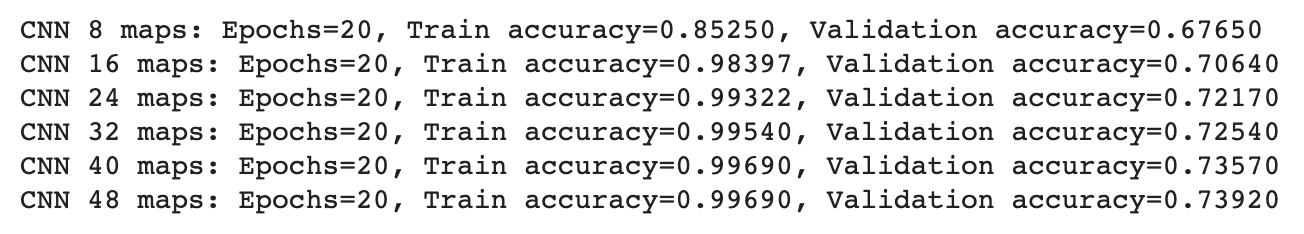
\includegraphics[width=\textwidth]{images/featuremap_result}
		\caption{Genauigkeitsmetriken unterschiedlicher Feature-Map Größen}
		\label{fig:featuremap_results}
	\end{subfigure}\hfill%
	\begin{subfigure}[ht]{.9\textwidth}
		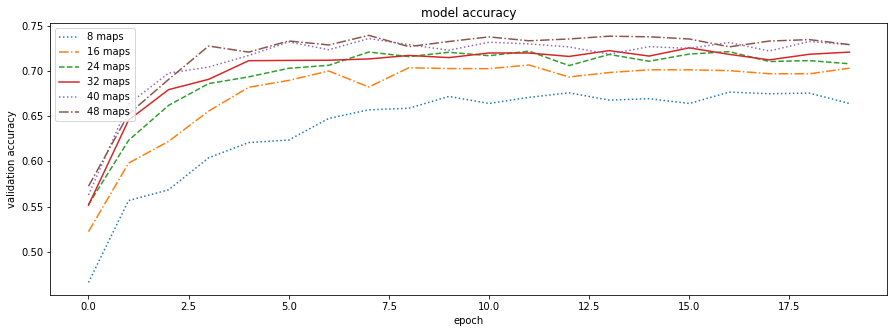
\includegraphics[width=\textwidth]{images/featuremap_result_graph}
		\caption{Grafische Darstellung der Genauigkeitsmetriken}
		\label{fig:featuremap_graph_results}
	\end{subfigure}\hfill%
	\caption{Entscheidungsfindung Feature-Map Größe}
\end{figure}

\subsection{Bestimmung der Größe des Fully-Connected Layers}

In den vorherigen Schritten wurden Anpassungen ausschließlich an den Convolutional Layern vorgenommen. Im nächsten Schritt wird der Fully-Connected Dense Layer evaluiert, um eine Aussage über die in diesem Layer lokalisierten Neuronen treffen zu können. Um den Matrix-Output der Convolutional- und Pooling-Layer in einen Dense Layer speisen zu können, muss dieser zunächst ausgerollt werden \emph{(flatten)}. Die Positionsmerkmale gehen bei dieser Modifikation zwar verloren, jedoch werden die ortsunabhängigen Objektinformationen behalten, wodurch eine Übergabe in einen Output Layer mit passender Anzahl von Neuronen ermöglicht werden kann. Aktiviert werden die Neuronen im Dense Layer durch die \ac{ReLU} Funktion (siehe Kapitel \ref{sec:ann}). Zur ausführlichen Evaluierung werden erneut mehrere Netzwerke erstellt und auf die erzielte Leistung überprüft. 

\begin{itemize}
	\item 2432 - $[32C5-P2]$ - $[64C5-P2]$ - $[96C5-P2]$ - \textbf{0} - 10
	\item 2432 - $[32C5-P2]$ - $[64C5-P2]$ - $[96C5-P2]$ - \textbf{32} - 10
	\item 2432 - $[32C5-P2]$ - $[64C5-P2]$ - $[96C5-P2]$ - \textbf{64} - 10
	\item 2432 - $[32C5-P2]$ - $[64C5-P2]$ - $[96C5-P2]$ - \textbf{128} - 10
	\item 2432 - $[32C5-P2]$ - $[64C5-P2]$ - $[96C5-P2]$ - \textbf{256} - 10
	\item 2432 - $[32C5-P2]$ - $[64C5-P2]$ - $[96C5-P2]$ - \textbf{512} - 10
	\item 2432 - $[32C5-P2]$ - $[64C5-P2]$ - $[96C5-P2]$ - \textbf{1024} - 10
	\item 2432 - $[32C5-P2]$ - $[64C5-P2]$ - $[96C5-P2]$ - \textbf{2048} - 10
\end{itemize}

Abbildung \ref{fig:fullyconnected_results} und \ref{fig:fullyconnected_graph_results} geben Aufschluss darüber, welche Performance das Modell mit unterschiedlich großen Fully-Connteced Layern erzielt. Die Verwendung von 256 Neuronen erzielt die höchste Validierungsgenauigkeit, weshalb dieser Wert für die weitere Berechnung übernommen wird. 

\begin{figure}[htb]
	\centering
	\begin{subfigure}[ht]{.9\textwidth}
		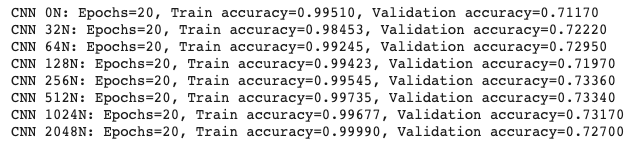
\includegraphics[width=\textwidth]{images/dense_metric}
		\caption{Genauigkeitsmetriken unterschiedlicher Fully-Connected Layer Größen}
		\label{fig:fullyconnected_results}
	\end{subfigure}\hfill%
	\begin{subfigure}[ht]{.9\textwidth}
		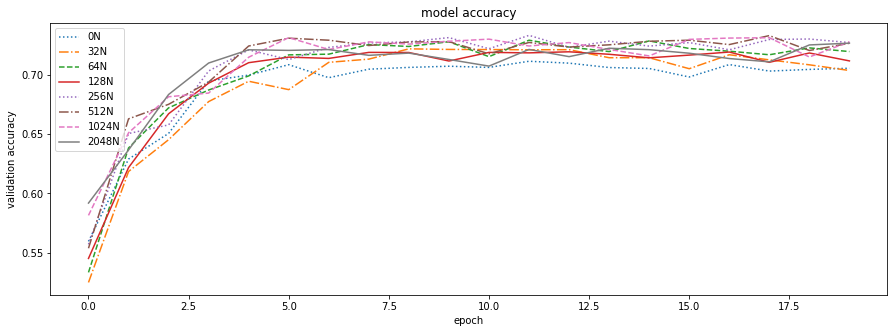
\includegraphics[width=\textwidth]{images/dense}
		\caption{Grafische Darstellung der Genauigkeitsmetriken}
		\label{fig:fullyconnected_graph_results}
	\end{subfigure}\hfill%
	\caption{Entscheidungsfindung Fully-Connected Layer Größe}
\end{figure}

\subsection{Ermittlung des Dropout Thresholds}

Dropout wird als Regularisierungsmethode eingesetzt um die Gefahr von Overfitting zu verringern. Hierfür wird eine vorher spezifizierte Anzahl von Neuronen in jedem Layer des Netzwerks ausgeschaltet (engl. dropout) und für die kommenden Berechnungsschritte ignoriert \cite[1929-1958]{JMLR:v15:srivastava14a}. Um den besten Dropout Wert zu ermitteln werden sieben Netzwerke trainiert, die jeweils ein Inkrement von 10\% besitzen. Als Nebeneffekt des Dropouts ist in Abbildung \ref{fig:dropout_results} und \ref{fig:dropout_graph_results} eine Schmälerung der Trainingsgenauigkeit zu beobachten. Da hierbei jedoch Overfitting reduziert wird, kann davon ausgegangen werden, dass die zuvor erzielten Genauigkeiten nur erzielt wurden, da das Netzwerk zu viele Informationen über die Bilddaten kannte. Währenddessen ist ein Anstieg der Validierungsgenauigkeit zu erkennen, was auf einen Erfolg der Overfitting Reduktion schließen lässt. Der Dropout Wert von 20\% wird anschließend für das finale Modell verwendet. 

\begin{figure}[htb]
	\centering
	\begin{subfigure}[ht]{.9\textwidth}
		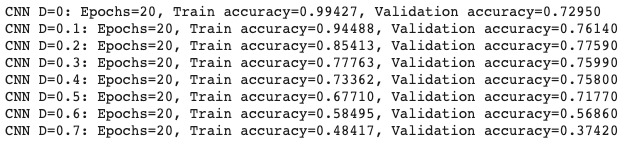
\includegraphics[width=\textwidth]{images/dropout}
		\caption{Genauigkeitsmetriken unterschiedlicher Dropout Layern}
		\label{fig:dropout_results}
	\end{subfigure}\hfill%
	\begin{subfigure}[ht]{.9\textwidth}
		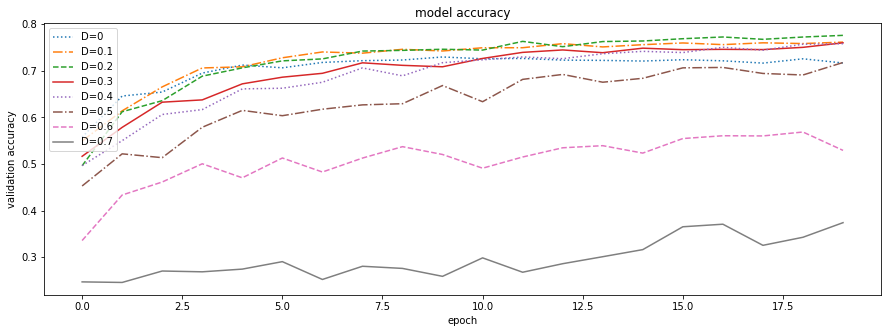
\includegraphics[width=\textwidth]{images/dropout_graph}
		\caption{Grafische Darstellung der Genauigkeitsmetriken}
		\label{fig:dropout_graph_results}
	\end{subfigure}\hfill%
	\caption{Entscheidungsfindung Dropout Threshold}
\end{figure}

\newpage

\section{Definition des finalen Modells}\label{sec:finalmodel}

Durch die in den vorherigen Kapiteln gewonnenen Erkenntnisse kann folglich ein finales Modell erstellt und mit dem initialen Modell verglichen werden. Das Modell setzt sich zusammen aus

\begin{itemize}
	\item 2432 - $[32C5-P2]$ - $[64C5-P2]$ - $[96C5-P2]$ - 256 - 10 
\end{itemize}

mit einem errechneten Dropout von 20\%.

\begin{figure}[htb]
	\centering
	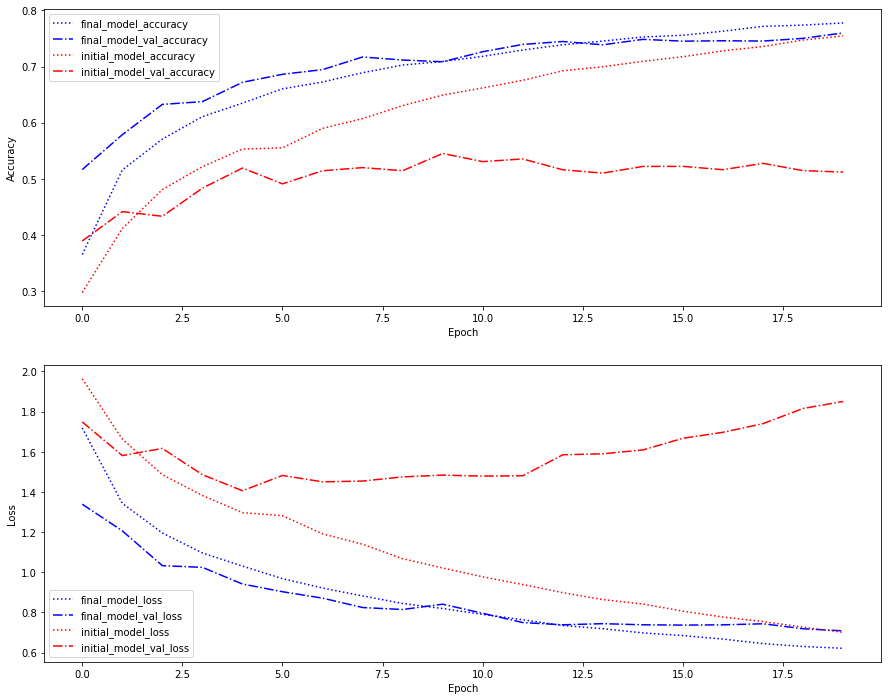
\includegraphics[width=\textwidth]{images/comparison_initial_final}
	\caption{Vergleich Initiales und Finales Modell}
	\label{fig:comparison_initial_final}
\end{figure}

Es ist zu erkennen, dass die initial errechnete Trainingsgenauigkeit eine viel geringere Abweichung zur Validierungsgenauigkeit aufzeigt. Selbiges ist bei der Berechnung des Verlusts zu erkennen, was auf einen Erfolg der Modelloptimierung schließen lässt. 
Abschließend ist zu erwähnen, dass dieses Modell einen Multi-class Anwendungsfall beschreibt. Für die ordnungsgemäße Verwendung ist die Transformation des Anwendungsfalles von Multi-class zu Multi-label benötigt. Die Erzeugung dieses Modells legt die theoretische Umsetzbarkeit hierfür dar. Die ausstehende Transformation ist in Kapitel \ref{sec:machine_learning} beschrieben.

